\chapter{Specifikace}

% strana 6 a 9
Sommerville~\cite{sommerville_softwareengineering_2011} uvádí fundamentální aktivity softwarového inženýrství: specifikace, vývoj, validace a evoluce.
Dále definuje softwarovou specifikaci jako aktivitu, při které zákazníci a inženýři definují software, který má být vyprodukován, a omezení na jeho provoz.

V~této kapitole definujeme software, který budeme tvořit, pomocí požadavků uživatele, případů užití, diagramu tříd v~konceptuální vrstvě a procesů.

\section{Požadavky}

Požadavky na softwarový systém jsou popisy toho, co by měl systém dělat -- služby, které poskytuje, a omezení na jeho provoz.
Tyto požadavky by měly reflektovat potřeby zákazníka na systém a jeho účel, uvádí Sommerville~\cite[s.~83]{sommerville_softwareengineering_2011}.

Požadavky na funkce systému nazýváme funkční.
Požadavky na provoz systému a jeho omezení nazýváme nefunkční.

Dále uvedeme vybrané funkční a nefunkční požadavky z~pohledu uživatele systému.

\subsection{Funkční požadavky}
\newlist{enumfp}{enumerate}{1}
\setlist[enumfp]{label=\textbf{FP\hyp{}\arabic*},ref=FP\hyp{}\arabic*}

\subsubsection*{Projekt}
\begin{enumfp}
  \item V~systému bude možné vytvořit nový projekt.
  \item Projekt bude možné uložit.
  \item Projekt bude možné načíst.
  \item Projekt bude možné pojmenovat pro odlišení od ostatních projektů.
  \item Jednotlivé diagramy bude možné exportovat do rastrového i vektorového formátu.
  \item Do těchto exportovaných formátů bude volitelně možné vložit projekt, který z~nich pak bude možné načíst.
  Tímto bude projekt možné otevřít jak v~prohlížeči obrázků (a zobrazit rastrově nebo vektorově diagram), tak v~našem systému a pokračovat v~práci.
  \item Zobrazení každého diagramu bude možné posouvat myší.
  \item Zobrazení každého diagramu bude možné přibližovat a oddalovat kolečkem myši.
  \item Posunutí a přiblížení bude volitelně možné synchronizovat mezi všemi diagramy.
  \item Systém bude kontrolovat validitu uživatelem vytvořených konstruktů.
\end{enumfp}

\subsubsection*{ER Diagram}
\begin{enumfp}[resume]
  \item Do diagramu bude možné přidat entitní typ.
  \item Do diagramu bude možné přidat vztahový typ.
  \item Do diagramu bude možné přidat atribut.
  \item Mezi entitním a vztahovým typem bude možné vytvořit spojení.
  \item Mezi entitním typem a atributem bude možné vytvořit spojení.
  \item U~spojení bude možné specifikovat a zobrazit kardinalitu.
  Dolní mez bude buď 0 nebo 1, horní mez 1 nebo $n$.
  Výchozí kardinality ($1..1$) nebudou zobrazeny.
  \item Bude možné vytvořit ISA hierarchii mezi entitními typy.
  \item Vlastnosti všech objektů bude možné měnit (popisky, typ, pozice).
  Tyto změny budou reflektovány v~ostatních diagramech.
  \item Objekty bude možné posunovat držením levého tlačítka myši a tažením.
  \item Všechny objekty bude možné zvolit levým tlačítkem myší.
  \item Při držení klávesy \keys{\ctrl} bude možné zvolit více objektů najednou postupným klikáním levého tlačítka myši.
  \item Veškeré objekty bude možné z~diagramu mazat alespoň klávesou \keys{Delete}.
  \item Uživatel bude moct využít předpřipravené konstrukty, které bude možné vložit do diagramu.
  Například se může jednat o~ISA hierarchie s~předpřipravenými entitami.
\end{enumfp}

\subsubsection*{Schématická kategorie}
\begin{enumfp}[resume]
  \item Objekty a morfismy schematické kategorie bude možné přidávat a mazat, přičemž tato změna se odrazí v~ostatních diagramech.
  \item V~diagramu se zobrazí data o~objektech a morfismech včetně kardinalit a popisků.
  Výchozí kardinality ($1..1$) se zobrazovat nebudou.
  \item Objekty bude možné posouvat a jejich posunutí se odrazí na ostatních diagramech.
  \item Při zvolení objektu se barevně vyznačí všechny objekty v~okolí, které ho identifikují (a jinou barvou identifikátory vzdálené).
\end{enumfp}

\subsubsection*{Vizualizace schematické kategorie}
\begin{enumfp}[resume]
  \item Vizualizace schematické kategorie ze schematické kategorie vytěží sémantiku a vizualizuje ji různými tvary.
  \item Při zvolení objektu se barevně zvýrazní bezprostřední a vzdálené identifikátory různými barvami.
\end{enumfp}

\subsection{Nefunkční požadavky}
\newlist{enumnfp}{enumerate}{1}
\setlist[enumnfp]{label=\textbf{NFP\hyp{}\arabic*},ref=NFP\hyp{}\arabic*}

\begin{enumnfp}
  \item Aplikaci bude možné používat na všech běžných desktopových operačních systémech.
  \item Nesmí dojít ke ztrátě práce při náhlém ukončení aplikace kvůli interním či externím vlivům.
  To může být zařízeno např. průběžným ukládáním práce.
  \item Aplikaci bude možné používat i při výpadku internetového připojení.
  \item V~rámci bezpečnosti žádná data týkající se práce na projektu neopustí zařízení klienta, pokud tak klient explicitně neučiní (například export a přesun souboru).
  \item Aplikace bude navržena tak, aby bylo možné bez větších komplikací rozšířit její funkcionalitu (např. přidat podporu UML).
\end{enumnfp}

\section{Diagram tříd}

V~této kapitole představíme konceptuální model.
Jedná se o~část světa, na kterou vymezujeme svůj diskurz.

Na obrázku~\ref{fig:class-diagram:diagram} je UML diagram tříd konceptuálního modelu diagramů.

Diagram konceptuálního modelu schematické kategorie lze pozorovat na obrázku~\ref{fig:class-diagram:schemcat}.

\begin{figure}[!htb]
  \centering
  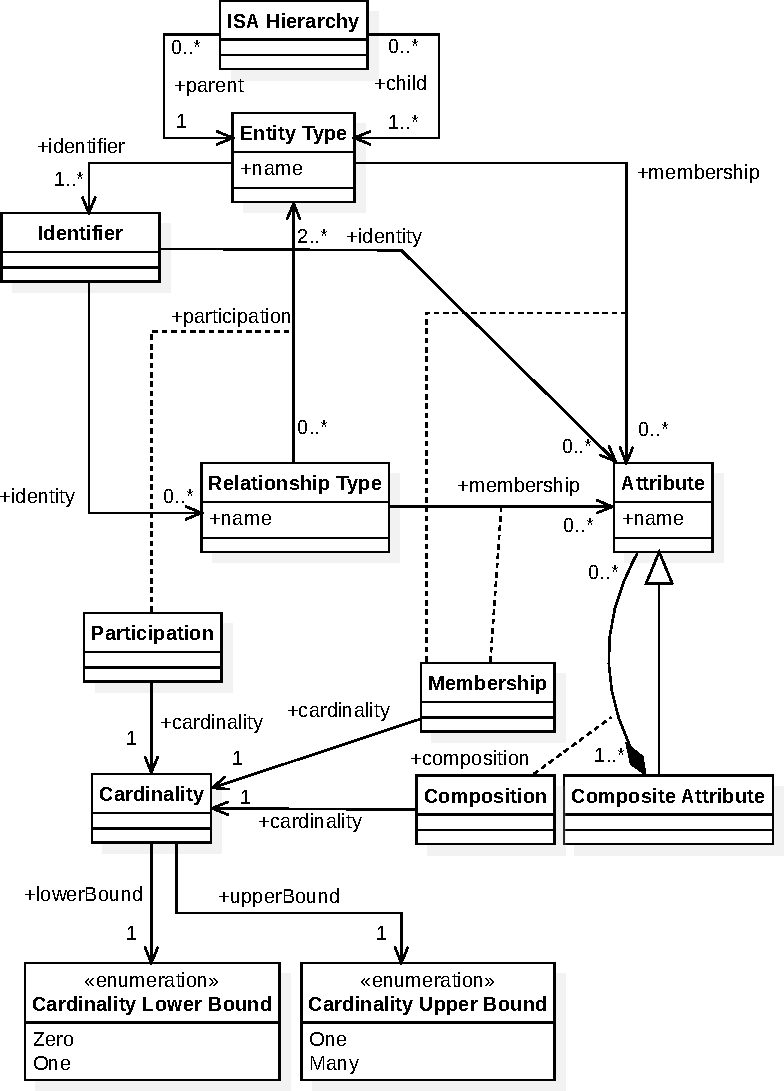
\includegraphics[width=\maxwidth{\textwidth}]{../img/diagrams/er-diagram-model.pdf}
  \caption{Diagram tříd -- ER diagram}
  \label{fig:class-diagram:diagram}
\end{figure}
\begin{figure}[!htb]
  \centering
  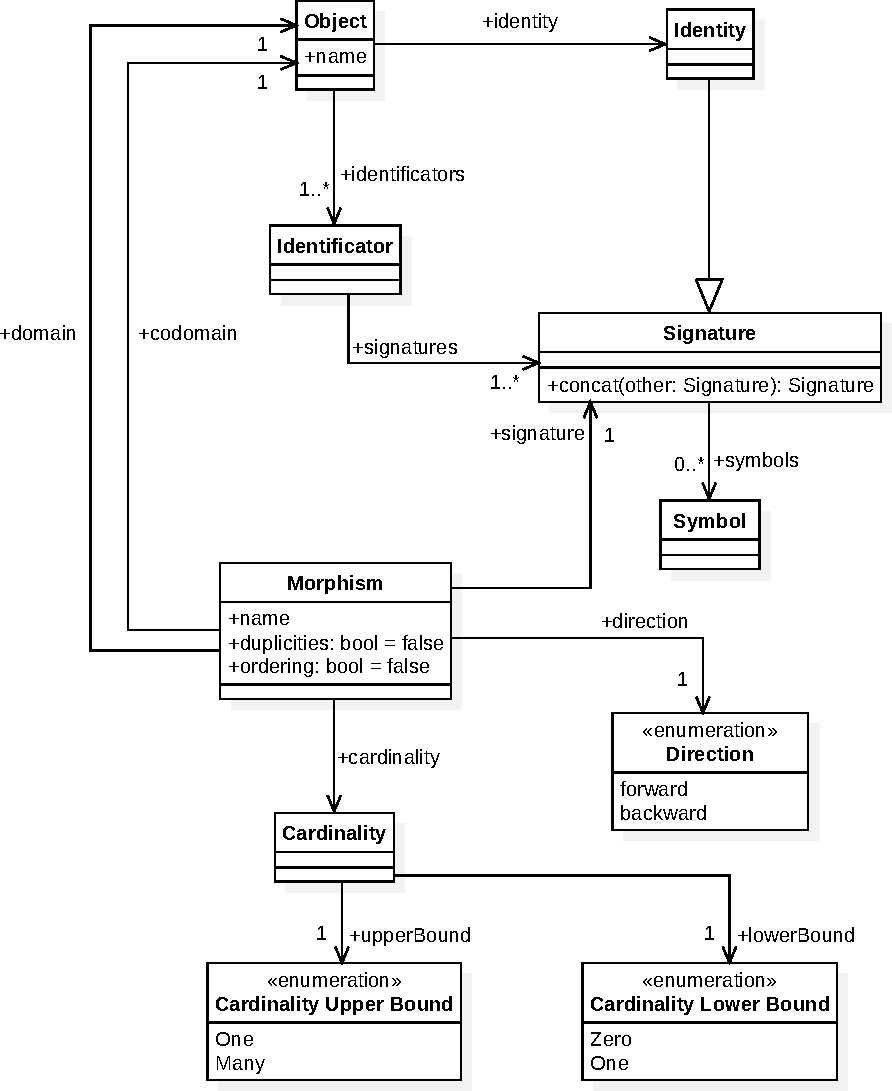
\includegraphics[width=\maxwidth{\textwidth}]{../img/diagrams/schema-category-model.pdf}
  \caption{Diagram tříd -- schematická kategorie}
  \label{fig:class-diagram:schemcat}
\end{figure}

